% =============================================================================
% timeline.tex — Horizontal timeline with annotated events
%
% Shows: a time axis with milestone markers above and explanatory annotations
% staggered below to avoid label collisions.
%
% Compiles standalone via: xelatex timeline.tex
% =============================================================================

\documentclass[border=4pt]{standalone}
\usepackage{tikz}
\usetikzlibrary{arrows.meta, decorations.pathreplacing}

\definecolor{axis}{HTML}{1A1A1A}
\definecolor{event}{HTML}{012169}
\definecolor{annot}{HTML}{B23A48}

% -----------------------------------------------------------------------------
% Diagram: horizontal timeline with 5 events.
% Coordinates (x = cm, 1 cm ≈ 6 months):
%   axis from (0, 0) to (12, 0)
%   E1 at (1.5, 0)   label "Policy A" above
%   E2 at (3.5, 0)   annotation below-left
%   E3 at (6.0, 0)   label "Reform" above
%   E4 at (8.5, 0)   annotation below-right
%   E5 at (11.0, 0)  label "Policy B" above
% Labels above events; annotation text below, staggered left/right to clear 0.3cm.
% -----------------------------------------------------------------------------

\begin{document}
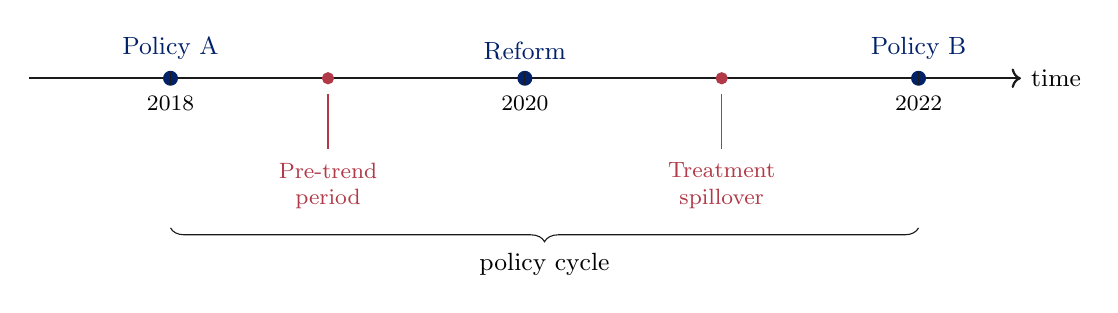
\begin{tikzpicture}
  % Axis
  \draw[->, thick, draw=axis] (-0.3, 0) -- (12.3, 0) node[right] {\small time};

  % Event markers + above-axis labels
  \foreach \x/\year/\lbl in {
    1.5/2018/{Policy A},
    6.0/2020/{Reform},
    11.0/2022/{Policy B}
  } {
    \filldraw[event] (\x, 0) circle (2.5pt);
    \draw[draw=axis, thin] (\x, -0.08) -- (\x, 0.08);
    \node[below, font=\footnotesize] at (\x, -0.1) {\year};
    \node[above, event, font=\small] at (\x, 0.12) {\lbl};
  }

  % Intermediate annotations (below, staggered down to 0.9cm)
  \filldraw[annot] (3.5, 0) circle (2pt);
  \draw[draw=annot, thin] (3.5, -0.2) -- (3.5, -0.9);
  \node[below, annot, font=\footnotesize, align=center] at (3.5, -0.95)
    {Pre-trend\\period};

  \filldraw[annot] (8.5, 0) circle (2pt);
  \draw[draw=annot, thin] (8.5, -0.2) -- (8.5, -0.9);
  \node[below, annot, font=\footnotesize, align=center] at (8.5, -0.95)
    {Treatment\\spillover};

  % Underlying era bracket
  \draw[decorate, decoration={brace, mirror, amplitude=5pt}, draw=axis]
    (1.5, -1.9) -- (11.0, -1.9);
  \node[below, font=\small] at (6.25, -2.1) {policy cycle};
\end{tikzpicture}
\end{document}
